\documentclass{standalone}

\usepackage{tikz}


\begin{document}
\begin{tikzpicture}
  \node (original) at (0, 0) {
    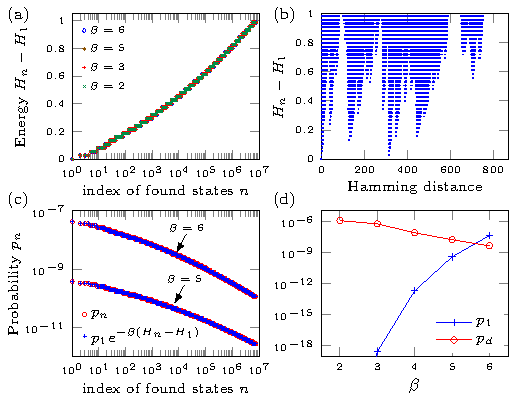
\includegraphics{tn-single-state}
  };

  \node[fill=white] at (-4, 3.15) {\small\textbf{a.}};
  \node[fill=white] at (-4, 0) {\small\textbf{c.}};
  \node[fill=white] at (0.5, 3.15) {\small\textbf{b.}};
  \node[fill=white] at (0.5, 0) {\small\textbf{d.}};

\end{tikzpicture}

\end{document}
